\chapter{Bayes Classifier}

\section{Introduction}

Bayes classification methods belong to the family of the oldest algorithms used
in machine learning. Principal ideas of Bayes (or sometimes called Bayesian)
classifiers are grounded in the works of a brilliant and famous English mathematician and statistician Thomas Bayes (1702, London - 1761, Tunbridge Wells,
United Kingdom). He was the first who used probability inductively and established a broadly applied mathematical basis for probability inference – a means
of calculating, from the number of times an event has occurred, the probability
that it may again occur in future trials or observations.

One characteristic and important property of the probabilistic computations
is that it works with uncertainty – probability very rarely returns an unequivocal
answer to a question. Hence, a typical solution is the selection of the answer with
the highest probability, taking into account that other possible answers might
sometimes be correct as well, according to the support provided by their degree
of probability.

Thomas Bayes’ findings on probability were published posthumously in the
Philosophical Transactions of the Royal Society of London as ‘Essay Towards
Solving a Problem in the Doctrine of Chances’ (1763). His discovery, also known
as Bayes’ theorem, is directed at practically solving various real-world problems.
The theorem not only addresses issues pertaining to Bayes’ times but modern
needs of data and information processing often take advantage of it as well often.

An interested reader may get acquainted with Thomas Bayes’ original article by accessing this URL \cite{ref19}. The article was communicated to John Canton,
M. A. and F. R. S., in Newington Green, in a letter by Mr. Richard Price on
November 10, 1763.

As an example related to text-mining, everyone who employs the commonly
used electronic mail communication is also likely to use a kind of so-called spam
filter, part of which is the implementation of a simplified form of Bayes’ theorem
widely known as na¨ıve Bayes classifier (see more in Subsection 5.4 mentioned
below). One of the big advantages of the Bayes classification methods is their excellent mathematical foundation in probability theory, particularly in conditional
probability modeling.

Such models are generally applicable to any task where the knowledge represented by the probabilities of being a member of a certain class is acceptable,
provided that a solved problem is described by training data supporting and enabling probability calculations. (A reminder that training data is a set of examples where the classification is known for each example.) Those probabilities can
then play a role of weights, backing individual class memberships – a knowledge
miner may select a hypothesis having the highest support.

It is necessary to keep in mind the fact that Bayes inference methods do not
generally provide crisp, unequivocal answers of the type 
‘an unlabeled event $a_i$ belongs just to a class $C_j$ with the probability 
$p(a_i) = 1.0$ and certainly not to another class $C_{k}$, $k \neq j$’. 
Usually, for such a probability $p(a_i)$, it holds true that
$
0.0 < p(a_i) < 1.0,
$
even if either $p(a_i) = 0.0$ or $p(a_i) = 1.0$ is also quite possible
but not typical in practice.

\section{Bayes' Theorem}

Bayes’ theorem is an interesting way to present, in more detail, the application
of the probability theory to machine learning because this theory often plays, at
least ‘just’ in the background, one of the fundamental roles in many algorithms.
There are many good books that can be recommended to familiarize a reader with
mathematical details, applications, and implementations of Bayesian methods.
Deeper knowledge may be found, for example, in \cite{ref23, ref100, ref160, ref191, ref129, ref29} or
many others available from assorted authors and publishers propounding various
point of views, sometimes focused more on theory, at others more on practice.

The principle of Bayes’ theorem can be simply explained using two events
(sometimes called propositions) labeled a and b, each having affiliated definitions:

\begin{itemize}
    \item $p(a)$ – an unconditional a priori probability of $a$ without any regard to $b$,

    \item $p(b)$ – an unconditional a priori probability of $b$ without any regard to $a$,

    \item $p(a \mid b)$ – a conditional probability of observing an event $a$ given that $b$ is true, i.e., $p(b) = 1.0$, and

    \item $p(b \mid a)$ – a conditional probability of observing an event $b$ given that $a$ is true, i.e., $p(a) = 1.0$,
\end{itemize}

where any probability $p(\cdot)$ is defined within the real interval 
$
0.0 \le p(\cdot) \le 1.0.
$
The probabilities of events are typically computed from their observed frequencies – a posteriori probabilities, which is quite natural for real-world practical
problems. Further, using the known product rule that both $a$ and $b$ must occur
together while the order of their occurrence is insignificant, that is, $a \wedge b = b \wedge a$,
it is possible to write:

\begin{align}
p(a \wedge b) &= p(a \mid b) \, p(b), \label{eq:5.1} \\
p(b \wedge a) &= p(b \mid a) \, p(a). \label{eq:5.2}
\end{align}

Note: a and b are two events that are generally not mutually independent.

Because the left sides of Eq. 5.1 and Eq. 5.2 describe the same event combination (logical conjunction a AND b), it is possible to write the following equation
using the right side equality of Eq. 5.1 and Eq. 5.2:

\begin{equation}
p(a \mid b) \, p(b) = p(b \mid a) \, p(a). \label{eq:5.3}
\end{equation}

After dividing both sides of the formula Eq. 5.3 by p(b), a new equation
Eq. 5.4 can be acquired, which is that famous Bayes’ rule or Bayes’ theorem:

\begin{equation}
p(a \mid b) = \frac{p(b \mid a) \, p(a)}{p(b)}, \quad p(b) > 0. \label{eq:5.4}
\end{equation}

What does Eq.~\eqref{eq:5.4} actually say? The result, i.e., the enumerated left side 
$p(a\mid b)$, provides the a posteriori probability of $a$ given some observation of $b$.

The theory of probability can be used for extending the theorem to more than
two events; however, the general computational complexity rapidly grows nonlinearly, demanding the enumeration of many formula members. This is a disadvantage of Bayes’ theorem, namely when it is applied to large spaces with a very
high number of dimensions $x_i$ (which is typical for text mining where a term
from a vocabulary represents a dimension).

Fortunately, there is a practical, even if not quite mathematically correct, solution known as na¨ıve Bayes classifier mentioned in the following section – and
it has been successfully used for a long time in many practical real-world areas,
including text mining.

It is also possible to look at the problem from this perspective: Let $D$ stand
for a set of collected data items (that is, all available observations up to a certain
time), and $h_i \in H$ for an $i$-th hypothesis from a set $H$ of $n$ various hypotheses that
are, to a certain degree, supported by that data, where $1 \le i \le n$.

The equation Eq. 5.5 can now be written in the following way:

\begin{equation}
p(h_i \mid D) = \frac{p(D \mid h_i) \, p(h_i)}{p(D)}, \quad p(D) > 0. \label{eq:5.5}
\end{equation}

The question is: Which of the hypotheses has the highest support (that is,
probability value) given that data D is functioning as an empirical proof for a correct final decision? Bayes’ theorem provides a way to calculate the a posteriori
probability of each hypothesis hi
, usually referred to as a maximum a posteriori
(MAP) hypothesis, hMAP, which is defined using the following equation:

\begin{equation}
h_{\text{MAP}} = \arg\max_{h \in H} p(h \mid D). \label{eq:5.6}
\end{equation}

Using Eq.~\eqref{eq:5.5} and omitting $p(D)$ from its denominator (because it has the
same value for each $h_i \in H$):

\begin{equation}
p(h_i \mid D) \propto p(D \mid h_i) \, p(h_i). \label{eq:5.7}
\end{equation}

Then, applying Eq. 5.7 to simplify Eq. 5.6, the latter can now be rewritten as
a proportional relationship:

\begin{equation}
h_{\text{MAP}} \propto \arg\max_{h \in H} p(D \mid h) \, p(h). \label{eq:5.8}
\end{equation}

The most probable classification of a new, unlabeled instance can be obtained
by combining the prediction of all hypotheses that are weighted by their posterior
probabilities.

The question which arises is, how the previous equations can be used for
inductive machine learning and supervised classification based on training using
labeled samples.

In his book \cite{ref199}, the author Tom Mitchell demonstrates a nice example when 
$h_{\text{MAP}}$ may not provide the correct answer (suggesting ‘a positive result’), which
is supported by its a posteriori probability, let us say, 0.4 because the other two hypotheses together suggest ‘a negative result’ (let us say, probabilities 0.3 and 0.3,
i.e., together 0.6) and therefore their combined a posteriori probabilities outperform $h_{\text{MAP}}$.

\section{Optimal Bayes Classifier}

To determine the strongest support of a hypothesis, it is necessary to combine
the predictions of all hypotheses, weighted by their a posteriori probabilities. Let
$C$ be a set of possible $m$ classes, $c_j$, $2 \le j \le m$, such that $c_j \in C$. The goal is to
find the best classification $c_j$ supported by the observed data $D$, that is, having
the highest conditional probability $p(c_j \mid D)$, which can be computed in this way:

\begin{equation}
p(c_j \mid D) = \sum_{h_i \in H} p(c_j \mid h_i) \, p(h_i \mid D). \label{eq:5.9}
\end{equation}

In such a case, the most probable class-label assignment, $c_j$,
to an unlabeled item is given by the maximum value of $p(c_j \mid D)$:

\begin{equation}
c_j = \arg\max_{c_j \in C} \sum_{h_i \in H} p(c_j \mid h_i) \, p(h_i \mid D). \label{eq:5.10}
\end{equation}

Note: argmax returns a class label, which is supported by the highest value
of computed conditional probability.

\section{Na\"ive Bayes Classifier}

According to theory, the optimal Bayes classifier provides the best possible classification result based on given data and hypotheses. Unfortunately, in practice,
the calculation – the sum of all multiplications – of all necessary combinations in
Eq. 5.9 or Eq. 5.10 might be very demanding from the computational complexity
point of view.

This is especially (but not only) true in text mining because assigning a correct class-label $c_j$ depends on the number of attributes, which here are words
in social-media contributions or text documents. After collecting a big number
of training samples (which is good from the probability computation point of
view), their vocabulary may be very large – thousands or tens of thousands unique
words (or generally terms).

Each word has its probability in every class and there are very many possible
attribute combinations, even if the data is reduced by, for example, eliminating
insignificant terms.

Let $a_1, a_2, \dots, a_N$ be the given attributes (vocabulary words). Then, using
Eq.~5.8, it is possible to write for the best classification, $c_{\text{MAP}}$:

\[
c_{\text{MAP}} = \arg\max_{c_j \in C} \; p(a_1, a_2, \dots, a_N \mid c_j) \, p(c_j) \;. \tag{5.11}
\]

For large values of $N$, the computational complexity is given by the item
$p(a_1, a_2, \dots, a_N)$ in Eq.~5.11. Because of the possible mutual conditional dependence of attributes, it is necessary to compute probabilities of all their possible
combinations for a given $c_j$.

The idea of the so-called na\"ive Bayes classifier, which is (theoretically not quite
accurately) based on an assumption that there is no interdependence between
the attributes (which is that `na\"ivety') resulted as a way to make the computation
easier and practically applicable. It means that, for the classification, it is possible to employ a simpler equation to determine $c_{\text{MAP}}$, which can be called $c_{\text{NB}}$ (for NB like na\"ive Bayes):

\[
c_{\text{NB}} = \arg\max_{c_j \in C} \; p(c_j) \prod_i p(a_i \mid c_j) \;. \tag{5.12}
\]

In other words, using the probabilities of attributes in the training data, just
the product of a posteriori probabilities of observed attributes times a priori
probability of a class occurrence per classified textual item has to be calculated.
Due to that theoretical incorrectness, the classification result may be more frequently wrong, depending on how much the independence assumption is violated. More detailed explanations of the above-mentioned problems may be
found in \cite{ref199}, which inspired the description of optimal Bayes’ and na¨ıve
Bayes’ classifier.

Despite the incorrectness, the na¨ıve Bayes classifier is very popular because
its results are quite acceptable in thousands of existing applications. The reason
is that, in practice, usually only small fragments of attributes are somehow mutually dependent, if any. However, one should be watchful when interpreting the
classification results – this incorrectness may be one of the reasons for the occasional wrong classification which users of e-mail know well: non-spam labeled
as spam and vice versa.
\section{ Illustrative Example of Na"ıve Bayes}

In conclusion, the following, absolutely simplified example with limited data just
for demonstration, illustrates how the na¨ıve Bayes’ classifier works. Let the training data set be composed of seven sentences that express various descriptions of
weather, a ‘good/bad weather’ problem.

Each sentence (a weather report) belongs to either a positive class $\oplus$ (good
weather) or to a negative class $\ominus$ (bad weather) according to a certain categorization (let us say that warm is generally preferred to cold). This data set (using
only lower case letters) is used for training the na\"ive Bayes' classifier:

\begin{enumerate}
    \item it is nice weather $\oplus$
    \item it is cold $\ominus$
    \item it is not very cold $\oplus$
    \item not nice $\ominus$
    \item very cold $\ominus$
    \item cold $\ominus$
    \item very nice weather $\oplus$
\end{enumerate}

The csv format of the training samples may, in a well arranged way with
superfluous spaces, look like this (the numbers represent frequencies of words in
documents):

\begin{verbatim}
it, is, nice, weather, cold, not, very, class
1, 1, 1, 1, 0, 0, 0, pos
1, 1, 0, 0, 1, 0, 0, neg
1, 1, 0, 0, 1, 1, 1, pos
0, 0, 1, 0, 0, 1, 0, neg
0, 0, 0, 0, 1, 0, 1, neg
0, 0, 0, 0, 1, 0, 0, neg
0, 0, 1, 1, 0, 0, 1, pos
\end{verbatim}

Based on the knowledge obtained by generalization of the training samples,
the classifier is expected to answer a question: Which label should be assigned
to an unlabeled item it is not nice cold at all – a positive or negative one? What
would a human being say? Probably negative because the proposition it is not
nice cold at all does not sound as something positive from the semantic point
of view, especially for people who like warm weather. However, what would be
an answer from a computer equipped with a text-mining tool based on the na¨ıve
Bayes’ classifier?

First, it is necessary to compute the required probabilities using the frequencies of words $w_i$, $i = 1,2,\dots,7$, in the available training collection of samples:


\begin{itemize}
\renewcommand{\labelitemi}{}
    \item $w_1 = \text{it}$: 2 occurrences in $\oplus$, 1 occurrence in $\ominus$, in total 3
    \item $w_2 = \text{is}$: 2 occurrences in $\oplus$, 1 occurrence in $\ominus$, in total 3
    \item $w_3 = \text{nice}$: 2 occurrences in $\oplus$, 1 occurrence in $\ominus$, in total 3
    \item $w_4 = \text{weather}$: 2 occurrences in $\oplus$, 0 occurrence in $\ominus$, in total 2
    \item $w_5 = \text{cold}$: 1 occurrence in $\oplus$, 3 occurrences in $\ominus$, in total 4
    \item $w_6 = \text{not}$: 1 occurrence in $\oplus$, 1 occurrence in $\ominus$, in total 2
    \item $w_7 = \text{very}$: 2 occurrences in $\oplus$, 1 occurrence in $\ominus$, in total 3
\end{itemize}

The vocabulary contains 7 unique words: \textit{it, is, nice, weather, cold, not, very}. 
In total, the training set consisting of 7 documents contains 20 words altogether 
(12 for $\oplus$ and 8 for $\ominus$); some words are repeated several times.


One problem can be seen: the analyzed item it is not nice cold at all includes
two words at and all, which are not in the training set. In such a case, it is necessary to discard such words and work only with those that are in the training
vocabulary.

Later, if the classification looks quite correct, the classifier can be retrained
using the added labeled example(s) and the vocabulary can be correspondingly
extended – such a procedure used to be applied in semi-supervised learning (progressively building a larger training set to improve a classifier’s results).

Now, at all will be discharged here, leaving just it is not nice cold for the
classification.

Based on words in the classified item and their statistical values from the 
vocabulary, provided that the occurrences of words are mutually independent 
(which may or may not be entirely correct), the naive Bayes classifier gives an answer: 
the decision of assigning either $\oplus$ or $\ominus$ to the unlabeled item is based on 
computing the probabilities $p_{\text{NB}+}$ and $p_{\text{NB}-}$, respectively, 
whether the item belongs to $\oplus$ or $\ominus$:

\[
p_{\text{NB}+}(\text{it, is, not, nice, cold} \mid \oplus) =
p(\text{it} \mid \oplus) \, 
p(\text{is} \mid \oplus) \, 
p(\text{not} \mid \oplus) \, 
p(\text{nice} \mid \oplus) \, 
p(\text{cold} \mid \oplus)
\]

and

\[
p_{\text{NB}-}(\text{it, is, not, nice, cold} \mid \ominus) =
p(\text{it} \mid \ominus) \,
p(\text{is} \mid \ominus) \,
p(\text{not} \mid \ominus) \,
p(\text{nice} \mid \ominus) \,
p(\text{cold} \mid \ominus) \,.
\]

The a priori probability of being in the class $\oplus$ is $p(\oplus) = \frac{3}{7} \approx 0.429$ 
(3 positive sentences from a total of 7), and similarly, 
for the class $\ominus$, $p(\ominus) = \frac{4}{7} \approx 0.571$ 
(4 negative sentences from a total of 7).

Using all the known probabilities from the frequencies, everything is now
ready for the computation of the classification supporting-weights 
$\mathcal{P}_{\text{NB}}(\ominus)$ and $\mathcal{P}_{\text{NB}}(\oplus)$ 
for each class $c_1 = \ominus$ and $c_2 = \oplus$, 
where $c_1, c_2 \in C = \{c_1 = \ominus, c_2 = \oplus\}$, 
as requested by the naive Bayes classifier according to Eq.~5.12:

$\mathcal{P}_{\text{NB}}(\oplus) = p(\oplus) \, p(\text{it} \mid \oplus) \, p(\text{is} \mid \oplus) \, p(\text{not} \mid \oplus) \, p(\text{nice} \mid \oplus) \, p(\text{cold} \mid \oplus)$
$= \frac{3}{7} \cdot \frac{2}{12} \cdot \frac{2}{12} \cdot \frac{1}{12} \cdot \frac{2}{12} \cdot \frac{1}{12}$
$= 0.429 \cdot 0.167 \cdot 0.167 \cdot 0.08 \cdot 0.167 \cdot 0.08$
$= 0.00001279$

and

$\mathcal{P}_{\text{NB}}(\ominus) = p(\ominus) \, p(\text{it} \mid \ominus) \, p(\text{is} \mid \ominus) \, p(\text{not} \mid \ominus) \, p(\text{nice} \mid \ominus) \, p(\text{cold} \mid \ominus)$
$= \frac{4}{7} \cdot \frac{1}{8} \cdot \frac{1}{8} \cdot \frac{1}{8} \cdot \frac{1}{8} \cdot \frac{3}{8}$
$= 0.571 \cdot 0.125 \cdot 0.125 \cdot 0.125 \cdot 0.125 \cdot 0.375$
$= 0.00005228$

Thus, the result (class label) is:

$c_{\text{NB}} = \arg\max_{c_j \in C} (\mathcal{P}_{\text{NB}}(\ominus), \mathcal{P}_{\text{NB}}(\oplus))$
$= \arg\max_{\{c_1 = \ominus, c_2 = \oplus\}} (5.228 \cdot 10^{-5}, 1.279 \cdot 10^{-5})$
$= \ominus$

Because $\mathcal{P}_{\text{NB}}(\ominus) > \mathcal{P}_{\text{NB}}(\oplus)$, 
the result is that the unlabeled item should obtain the label $\ominus$ 
and it belongs to the negative propositions, 
which corresponds with the human expectation briefly discussed above.

Note that the results $\mathcal{P}(.)$ do not directly provide probability values.

They are numerical values playing the role of weights and, as such, may be 
safely used for selecting a hypothesis $c_{\text{NB}}$: 
$p(.) \neq \mathcal{P}(.)$, however, $p(.) \propto \mathcal{P}(.)$.

Should it be—for any reason—necessary to express $\mathcal{P}_{\text{NB}}(.)$'s as probabilities $p_{\text{NB}}(.)$'s, 
it is possible to normalize both output numbers $\mathcal{P}_{\text{NB}}(.)$ 
within the closed probability interval $[0.0,1.0]$:

$$
p_{\text{NB}}(\ominus) = \frac{\mathcal{P}_{\text{NB}}(\ominus)}
{\mathcal{P}_{\text{NB}}(\oplus) + \mathcal{P}_{\text{NB}}(\ominus)}, and \
p_{\text{NB}}(\oplus) = \frac{\mathcal{P}_{\text{NB}}(\oplus)}
{\mathcal{P}_{\text{NB}}(\oplus) + \mathcal{P}_{\text{NB}}(\ominus)}.
$$

After substituting appropriate numbers for symbols, the result is expressed
with the requested probabilities. In this case, the probability of being bad weather
is approximately four times higher than that of being good weather, thus the
result is well supported and quite acceptable:

$p_{\text{NB}}(\ominus) = 0.00005228 / (0.00005228 + 0.00001279) \approx 0.8034$,  
$p_{\text{NB}}(\oplus) = 0.00001279 / (0.00005228 + 0.00001279) \approx 0.1966$

$p_{\text{NB}}(\ominus) + p_{\text{NB}}(\oplus) = 0.8034 + 0.1966 = 1.0$.

As a reader may see, there are, in fact, two possible results that can be true; 
however, neither of them is fully true because neither $p_{\text{NB}}(\ominus)$ 
nor $p_{\text{NB}}(\oplus)$ are equal to 1.0. Therefore, the result is subject to 
uncertainty and a user has to decide which value is worth consideration. 
In reality, the result with the highest probability is typically selected, which is reasonable; 
however, a user can expect that such a system would not always work without occasional errors, 
even if the output would mostly be correct. If $p_{\text{NB}}(\ominus) = p_{\text{NB}}(\oplus)$, 
then the class can be selected randomly (the highest uncertainty, an indecisive case).

People who use electronic mail with a spam filter know it well: sometimes,
a message is not spam but is considered to be, and vice versa. The reason is that
the positive and negative class usually share many words (terms, phrases) like in
the example presented above – and the bag-of-words representation, which uses
separated individual words without their mutual relationships, introduces part of
that uncertainty. A word bad (or nice) can be in both the positive and the negative
class and even the combination of their probabilities does not entirely remove the
uncertainty. Sometimes it could also be difficult for human beings – as a reader
is likely to know.

In conclusion, one technical note. When computing the resulting probability
by multiplication of many individual probabilities, there is a danger of numerical
underflow, especially for classification of text documents using a broad vocabulary because the average probability value of a word is very low. That is why
such data-mining tools, instead of working with multiplication, employ summarization of logarithms of probability values.

\section{Naive Bayes Classifier in R}

The system R offers several implementations of the na¨ıve Bayes classifier. An
implementation which will be installed into R library, naivebayes, is briefly described in this section along with an example demonstrating how to use it for
text mining.

\subsection{Running Naıve Bayes Classifier in RStudio}

For simplicity, let us use one directory for data (in which there is for demonstration, the input file, BookReviews1000.csv, containing 1000 samples for training
and testing) as well as the R-code for running the na¨ıve Bayes classifier.

In the first step, RStudio is started and the source R-code is open. After clicking on the RStudio menu button Session, the selection of Set Working Directory
and finally To Source Location defines the working directory, where source inputs are found and where prospective outputs will be stored.

Console confirms this selection. For example:

\begin{verbatim}
> setwd("D:/R Book/Naive Bayes")
\end{verbatim}

The source code should run on clicking the button, Source.

If the package naivebayes has never been employed, there may be a red
error message:

\begin{verbatim}
Error in library (naivebayes) : there is no package
called ‘naivebayes’
\end{verbatim}

This is likely because the R library (which is one of the directories where R is
installed) does not implicitly contain such a package. In this case, it is necessary
to install naivebayes, which is quite simple as is illustrated in Figure 5.1:

\begin{enumerate}
    \item click Packages
    \item click Install
    \item write the package name naivebayes into the pop up window
    \item select Install dependencies (if not selected by default)
    \item click Install in the pop up window
\end{enumerate}

That is all that is required; the R-system will automatically install everything
necessary. The list of all installed libraries can be seen in RStudio under the
System Library label. After successful installation, the na¨ıve Bayes classifier can
run as described as follows (text lines can be wrapped when they are longer than
the available page width, and the wrapped part are indented – console messages
and R-code including comments – but actually they create just one line!).

\begin{figure}[H]
\centering
\begin{minipage}{0.9\textwidth}
    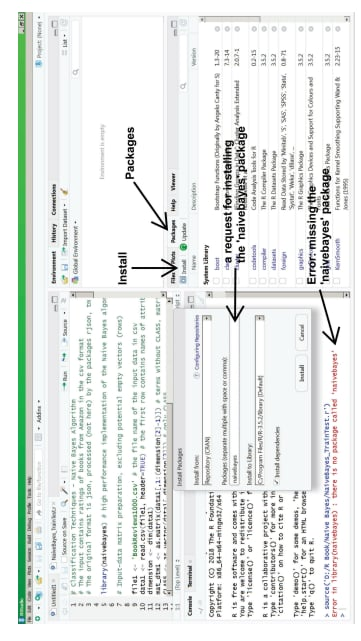
\includegraphics[width=\linewidth]{chapter/chapter5/figure5.1.jpg}
\end{minipage}%
\hspace{0.5em}%
\begin{minipage}{0.05\textwidth}
    \rotatebox{90}{\textbf{Figure 5.1:} Installing the package, \texttt{naivebayes}, for the naive Bayes classifier in RStudio from the Internet.}
\end{minipage}
\end{figure}


\subsection{Testing with an External Dataset}

This section illustrates possible R-code for generating and testing a trained na¨ıve
Bayes classifier using an extra test data-set. In this case, the simple approach is
applied just for the demonstration. In a matrix with 1000 samples, 100 randomly
selected positive and negative samples are taken for testing, and the remaining
900 for training. Each row in the matrix contains a randomly selected sample, the
sequence of which is also random from the class point of view, so it would not be
necessary to resample it randomly again. The selected 100 testing rows contain
48 positive samples and 52 negative ones, and the remaining, training samples,
452 positive and 448 negative ones, which is almost the ideal ratio, 50\% : 50\%.

Here is the sample R-code:

\begin{verbatim}
library(naivebayes)
# loading the data
data <- read.csv("BookReviews.csv", header=TRUE)
# converting the data to a matrix
dtm <- as.matrix(data)
# removing the object data (unnecessary from now)
rm(data)
# number of instances
n <- dim(dtm)[1]
# number of attributes
m <- dim(dtm)[2]
# indexes of 100 testing samples
number_of_test_samples <- 100
test_index <- sample(n, number_of_test_samples)
# selecting training samples
train_data <- dtm[-test_index, 1:(m-1)]
train_labels <- dtm[-test_index, m]
# selecting testing samples
test_data <- dtm[test_index, 1:(m-1)]
test_labels <- dtm[test_index, m]
# training a Naive Bayes model
nb_model <- naive_bayes(x=train_data, y=train_labels)
# calculating class predictions
predictions <- predict(nb_model, test_data, type="class")
# creating a confusion matrix
cm <- table(test_labels, predictions)
print("Confusion matrix")
print(cm)
# number of instances
n <- sum(cm)
# number of correctly classified instances for each class
correct <- diag(cm)
# numbers of instances in each class
instances_in_classes <- apply(cm, 1, sum)
# numbers of each class predictions
class_predictions <- apply(cm, 2, sum)
# accuracy
accuracy <- sum(correct)/n
# precision per class
precision <- correct/class_predictions
# recall per class
recall <- correct/instances_in_classes
# F1-measure per class
f1 <- 2 * precision * recall / (precision + recall)
# printing summary information for all classes
df <- data.frame(precision, recall, f1)
print("Detailed classification metrics")
print(df)
print(paste("Accuracy:", accuracy))
# macroaveraging
print("Macro-averaged metrics")
print(colMeans(df))
# microaveraging
print("Micro-averaged metrics")
print(apply(df, 2, function (x)
weighted.mean(x, w=instances_in_classes)))
The console output after a successful run:
[1] "Confusion matrix"
predictions
test_labels 0 1
0 38 14
1 9 39
[1] "Detailed classification metrics"
precision recall f1
0 0.8085106 0.7307692 0.7676768
1 0.7358491 0.8125000 0.7722772
[1] "Accuracy: 0.77"
[1] "Macro-averaged metrics"
precision recall f1
0.7721798 0.7716346 0.7699770
[1] "Micro-averaged metrics"
precision recall f1
0.7736331 0.7700000 0.7698850
\end{verbatim}

\subsection{Testing with 10-Fold Cross-Validation}

As another example for the same data, the code uses a standard 10-fold crossvalidation to gradually test the classifier accuracy.

There are 10 steps, each one uses 10\% of the samples for testing and 90\% for
training, and every sample gradually takes part in both sections. Classification
performance metrics are calculated at each step. Their final value is given by the
mean value of all 10 measurements. In our example, only the values of accuracy
are considered for simplicity. The standard error of the mean (SEM) that is used
in statistics for expressing an average error for different randomly selected testing
samples from a data population (an error generalization for the whole population)
is also calculated.

Given below is the sample R-code. A reader would notice that the code for
cross-validation testing is very similar to the code using a test set for testing. In fact, the same steps (selecting the data, building a model, using the model,
evaluating the model) are repeated ten times. In each iteration, different training
and test sets are created. Classification performance measures are calculated in
each iteration and the results are averaged at the end. To prevent repeating an
almost identical code in each chapter related to classification, the R code for
cross-validation testing is not included in the following chapters.

\begin{verbatim}
library(naivebayes)
# a function for calculating the standard error of the mean
sem <- function(x) sd(x)/sqrt(length(x))
# loading the data
data <- read.csv("BookReviews.csv", header=TRUE)
# converting the data to a matrix
dtm <- as.matrix(data)
# removing the object data (unnecessary from now)
rm(data)
# number of instances
n <- dim(dtm)[1]
# number of attributes
m <- dim(dtm)[2]
# 10 folds for cross-validation
number_of_folds <- 10
# marking samples in each of 10 folds with 1’s, 2’s, ..., 10’s
folds <- cut(1:n, breaks=number_of_folds, labels=FALSE)
# vector with accuracies
accuracies <- rep(0, times=number_of_folds)
for(i in 1:number_of_folds){
# selecting testing samples according to their fold-marks
test_index <- which(folds==i, arr.ind=TRUE)
# selecting training samples
train_data <- dtm[-test_index, 1:(m-1)]
train_labels <- dtm[-test_index, m]
# selecting testing samples
test_data <- dtm[test_index, 1:(m-1)]
test_labels <- dtm[test_index, m]
# training a Naive Bayes model
nb_model <- naive_bayes(x=train_data, y=train_labels)
# calculating class predictions
predictions <- predict(nb_model, test_data, type="class")
# obtaining a confusion matrix
cm <- table(test_labels, predictions)
# number of correctly classified instances for each class
correct <- diag(cm)
# numbers of each class predictions
class_predictions <- apply(cm, 2, sum)
# accuracy
accuracy <- sum(correct)/sum(cm)
# precision per class
precision <- correct/class_predictions
# printing the results
cat("Cross-validation fold: ", i, "\n",
" Accuracy: ", accuracy, "\n",
" Precision(positive): ", precision["1"], "\n",
" Precision(negative): ", precision["0"], "\n",
sep="")
# storing the accuracy for current crossvalidation fold
accuracies[i] <- accuracy
}
# printing the aggregated results from crossvalidation
cat("Average Accuracy: ",
round(sum(accuracies)/number_of_folds*100, 1), "%\n",
"SEM: ", round(sem(accuracies)*100, 2),
sep="")
Cross-validation fold: 1
Accuracy: 0.75
Precision(positive): 0.6666667
Precision(negative): 0.8478261
Cross-validation fold: 2
Accuracy: 0.67
Precision(positive): 0.6792453
Precision(negative): 0.6595745
Cross-validation fold: 3
Accuracy: 0.68
Precision(positive): 0.6521739
Precision(negative): 0.7419355
Cross-validation fold: 4
Accuracy: 0.75
Precision(positive): 0.6909091
Precision(negative): 0.8222222
Cross-validation fold: 5
Accuracy: 0.67
Precision(positive): 0.6323529
Precision(negative): 0.75
Cross-validation fold: 6
Accuracy: 0.67
Precision(positive): 0.6470588
Precision(negative): 0.71875
Cross-validation fold: 7
Accuracy: 0.64
Precision(positive): 0.5409836
Precision(negative): 0.7948718
Cross-validation fold: 8
Accuracy: 0.67
Precision(positive): 0.6515152
Precision(negative): 0.7058824
Cross-validation fold: 9
Accuracy: 0.64
Precision(positive): 0.6229508
Precision(negative): 0.6666667
Cross-validation fold: 10
Accuracy: 0.66
Precision(positive): 0.6716418
Precision(negative): 0.6363636
Average Accuracy: 68%
SEM: 1.24
\end{verbatim}

What are such results good for? The following point of view can be considered, for example, to summarize and somehow interpret the results. Each testing
subset for each of ten folds is classified using the particular na¨ıve Bayes model
created by available training samples. The standard error of the mean (SEM),
averaging classification errors for all individual random selections (each such
selection generally a has different error mean), is only 1.24\%. It is a good sign
when the SEM is small because of stability – it suggests that the created model
does not depend (too much) on different data samples and is stable.

Looking at individual fold results, it is obvious that negative examples have
lower classification errors than their positive counterparts (the same is valid also
for testing by the test data subset). This could be an interesting discovery, a kind
of dug out knowledge from the data, and an inspiration for subsequent research
(which is not included in this book). Why is it so?

A possible explanation might be that – after a closer exploration of words
and phrases in both data classes – the positive reviews are, for example, mutually more different (readers like more things) while the negative ones are more
homogeneous in terms of what readers dislike. In such a case, the generalization
of data (which might be the requested knowledge) may be more difficult for the
positive section and ‘positive’ readers might be separated into several ‘positive’,
more homogeneous, groups.

On the other hand, if there were many more (let us say, 95\%) training negative
reviews than positive ones (an unbalanced training set) – the conclusion might be
that a book is generally not very well accepted and its reprint would not pay off.
Or, that publishing of the next volume is not promising because all the previous
volumes did not demonstrate non-declining interest, and so on.





